% \documentclass[handout,aspectratio=43]{ctexbeamer}
\documentclass[aspectratio=43]{ctexbeamer}

\usepackage{unicode-math}
\usepackage{graphicx}
\usepackage{pdfpages}
\usepackage{hologo}
\usepackage{multicol}
\usepackage{booktabs}
\usepackage{fontspec}
\usepackage{bookmark}
\usepackage[outputdir=build]{minted}
\usepackage{xcolor}
\usepackage{hyperref}
\usepackage{cleveref}

\usetheme{Xiaoshan}

\author{45gfg9}

\makeatletter

\graphicspath{{lec4/}}

\usebackgroundtemplate{
    \ifnum\thepage>1
    \ifnum\thepage<\@abspage@last
    
\includegraphics[height=\paperheight]{background.png}
    \fi\fi
}

% PDF bookmark
\apptocmd{\beamer@@frametitle}{%
    \only<1>{\expandafter\ifnum\insertcontinuationcount<2\relax
    \bookmark[page=\the\c@page,level=4]{#1}\fi}}{}{}

\makeatother

\setbeamertemplate{frame numbering}{
    \tt\insertframenumber{} / \inserttotalframenumber{}
}
\setbeamerfont{alerted text}{series=\bfseries}

\metroset{
    progressbar=foot,
}

\setminted{
    breaklines,
    autogobble,
    fontsize=\small,
    style=xcode,
}

\hypersetup{
    unicode,
    pdfborder = {0 0 0},
    colorlinks,
    linkcolor = [HTML]{00008b},
    urlcolor = [HTML]{00008b},
}

\usefonttheme{serif,professionalfonts}
\setmainfont{LibertinusSerif}[
  Extension      = .otf,
  UprightFont    = *-Regular,
  BoldFont       = *-Bold,
  ItalicFont     = *-Italic,
  BoldItalicFont = *-BoldItalic]
\setmathfont{LibertinusMath-Regular.otf}
\setmonofont{JetBrains Mono}[
    UprightFont    = *-Light,
    BoldFont       = *-Medium,
    ItalicFont     = *-Light Italic,
    BoldItalicFont = *-Medium Italic,
    Scale          = 0.92]
\setCJKmainfont{Source Han Serif SC}[
    UprightFont    = * Light,
    BoldFont       = * Bold,
    ItalicFont     = * Medium,
    BoldItalicFont = * Bold,
    Scale          = 0.95,
    CharacterWidth = Full]
\setCJKmonofont{Source Han Sans SC}[
    AutoFakeSlant,
    Scale          = 0.92,
    CharacterWidth = Full]

\addtolength{\parskip}{0.5em}
\linespread{1.1}

\begin{document}


\includepdf{cover.png}

\section{Part.0 开始之前...}

\begin{frame}{本节内容}
\begin{itemize}
    \item 什么是 \LaTeX{}?如何编写和编译 \LaTeX{} 文档?
    \item \LaTeX{} 文档的基本结构与基础语法
    \begin{itemize}
        \item 文档结构、文档元素
        \item 文档类、宏包、环境、命令
        \item 标签、引用
    \end{itemize}
    \pause
    \item \LaTeX{} 的拿手好戏:数学公式
    \begin{itemize}
        \item 以及如何\textbf{正确}地编写数学公式
    \end{itemize}
    \item 写 \LaTeX{} 的尽头是套模板?
    \item 当遇到问题时,该去哪里寻求帮助
\end{itemize}
\end{frame}

\begin{frame}{如何自学本节内容} \label{how-to-learn}
\begin{itemize}
    \item 安装:\href{https://github.com/OsbertWang/install-latex-guide-zh-cn}{一份简短的关于 \LaTeX{} 安装的介绍}
    \item 学习:\href{https://github.com/CTeX-org/lshort-zh-cn}{一份(不太)简短的 \LaTeXe{} 介绍}(即 lshort)
        \begin{itemize}
            \item 或安装 TeX Live 后通过 \texttt{texdoc lshort-zh-cn} 命令打开
        \end{itemize}
    \item 其他参考:
        \begin{itemize}
            \item 符号大全:\href{https://www.ctan.org/pkg/comprehensive}{The Comprehensive \LaTeX{} Symbol List}
            \item 手写查询:\href{http://detexify.kirelabs.org/classify.html}{Detexify}
            \item \href{https://en.wikibooks.org/wiki/LaTeX}{\LaTeX{} Wikibook}
            \item \href{https://en.wikibooks.org/wiki/LaTeX/Mathematics}{\LaTeX{} Wikibook / Mathematics}
            \item \href{https://tex.stackexchange.com/}{\TeX{} - \LaTeX{} Stack Exchange}
            \item \href{https://www.learnlatex.org/en/}{Learn\LaTeX{}.org}
        \end{itemize}
    \item 速通本 slide Part.3 和 Part.5
\end{itemize}
\end{frame}

\section{Part.\texorpdfstring{$\boldsymbol{\varepsilon}$}{ε} 什么是 \LaTeX{}}

\begin{frame}{起源}
\begin{itemize}
    \item (1977) Donald Knuth 为排版《计算机程序设计艺术》而开始开发排版系统 \TeX{}
    \begin{itemize}
        \item 名称来源于希腊字母 $\tau\varepsilon\chi$,意为 technology
        \item 写作 TeX(注意大小写)
        \item 1978 年首次发布,目前的版本为 \TeX{} 3.141592653
    \end{itemize}
    \item (1984) Leslie Lamport 基于 \TeX{} 开发了 \LaTeX{}
    \begin{itemize}
        \item 写作 LaTeX(注意大小写),读作 /ˈleɪtɛk/
        \item \LaTeXe{} 成为目前最流行的 \TeX{} 宏集
    \end{itemize}
\end{itemize}
\end{frame}

\begin{frame}[fragile]{什么是 \LaTeX{} --- What you \emph{think} is what you get!}
\begin{columns}
\begin{column}{0.57\textwidth}
\onslide
\begin{minted}[fontsize=\tiny]{tex}
\documentclass{LALUbook}
\usepackage{amsmath}
% 省略一些内容……
\title{浙江大学 2023--2024 学年 \\ 线性代数荣誉课辅学讲义}
\author{2023--2024 学年线性代数 I/II(H)辅学授课 \\
        吴一航 \quad \verb|yhwu_is@zju.edu.cn|}
\begin{document}
% 省略一些内容……
\begin{example}
  \begin{enumerate}
    \item 已知椭圆$C:\dfrac{x^2}{4}+\dfrac{y^2}{3}=1$,
      若直线$l:y=kx+m$与椭圆$C$相交于$A,B$两点($A,B$
      不是左右顶点),且以$AB$为直径的圆过椭圆$C$的右顶点.
      求证:直线$l$过定点.
    \item 设$A_i\enspace(i=1,2,\ldots,n)$是$X$的子集.
      证明:$\overline{\displaystyle\bigcup_{i=1}^nA_i}
      =\displaystyle\bigcap_{i=1}^n\overline{A_i}$
      (其中集合上一横代表对全集$X$的补集).
  \end{enumerate}
\end{example}
% 省略一些内容……
\end{document}
\end{minted}
\end{column}
\onslide<2->
\begin{column}{0.43\textwidth}
    \begin{figure}
        \centering
        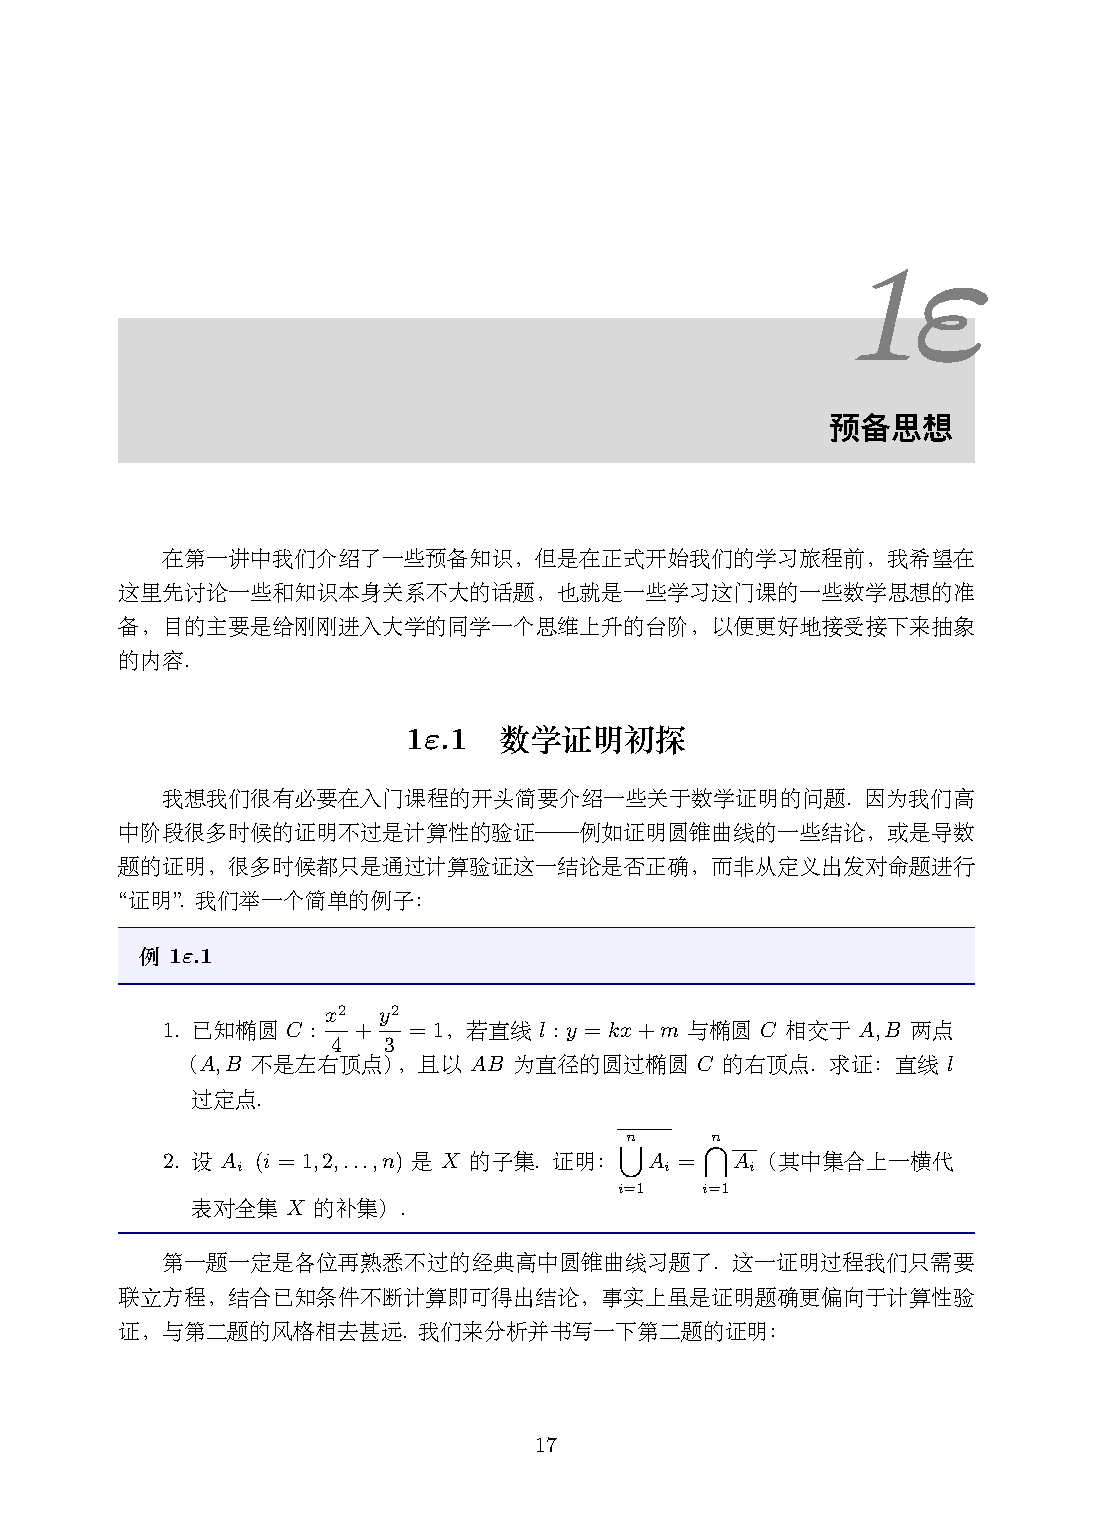
\includegraphics[width=\textwidth, trim={2cm 2cm 2cm 2cm}, clip]{lalu.pdf}
    \end{figure}
\end{column}
\end{columns}
\onslide
\scriptsize 来源:\href{https://github.com/yhwu-is/Linear-Algebra-Left-Undone}{线性代数:未竟之美}
\end{frame}

\begin{frame}{什么是 \LaTeX{} --- cont.}
\begin{itemize}
    \item 优点:专注于内容本身,排版效果好,公式排版强大,跨平台开源……
    \item 缺点:学习成本高,不容易排错,不容易定制样式,不所见即所得……
    \item 排版 vs. 文字处理?
    \begin{itemize}
        \item ``别把 \LaTeX{} 当 Word 用''
        \item \textbf{内容}与\textbf{样式}分离
        \item \alert{内容永远比样式重要}
    \end{itemize}
\end{itemize}
\end{frame}

\begin{frame}{关于发行版、引擎、编译指令}
\begin{itemize}
    \item 发行版即打包好的套装,包含引擎、宏包、字体、文档等
        \begin{itemize}
            \item 全平台:\TeX{} Live(推荐)、\hologo{MiKTeX}
            \begin{itemize}
                \item \href{https://mirrors.zju.edu.cn/CTAN/systems/texlive/Images/}{ZJU Mirror}
                \item \texttt{sudo apt install texlive-full}
            \end{itemize}
            \item macOS:Mac\TeX{},基本与 \TeX{} Live 一致
            \begin{itemize}
                \item \texttt{brew install --cask mactex}
            \end{itemize}
        \end{itemize}
    \pause
    \item 引擎即编译器,是编译 \TeX{} 代码生成文档的排版引擎
        \begin{itemize}
            \item 有 \TeX{}、\hologo{pdfTeX}、\hologo{XeTeX}、\hologo{LuaTeX}、\hologo{ConTeXt} 等
            \item 中文支持:\hologo{XeTeX}(推荐)、\hologo{LuaTeX}
        \end{itemize}
    \item 有两种语法,\hologo{plainTeX}(原始版本)和 \LaTeX{}
    \pause
    \item 编译指令根据引擎和格式来选择(类比 C 语言的编译)
        \begin{itemize}
            \item \texttt{latex}、\texttt{xelatex}、\texttt{lualatex} 等
            \item 推荐使用 \texttt{latexmk},自动选择编译指令
        \end{itemize}
\end{itemize}
\end{frame}

\begin{frame}{不想安装?}
\begin{itemize}
    \item \href{https://www.overleaf.com/}{Overleaf}:在线 \LaTeX{} 编辑器
    \item 云端服务更好用…吗?
    \item 多人协作、版本控制
    \pause
    \item 注意网络环境(咳咳)
\end{itemize}
\end{frame}

\begin{frame}{编写与编译}
\begin{itemize}
    \item 纯文本文件,后缀名为 \texttt{.tex}(类比 Markdown 的 \texttt{.md})
    \item 自带编辑器:TeXworks(TeX Live)、TeXShop(Mac\TeX{})
    \item \href{https://github.com/texstudio-org/texstudio}{TeXstudio}:跨平台的开源编辑器
    \item 谁说记事本就不行了?
    \pause
    \item 选择正确的编译指令
        \begin{itemize}
            \item 例如 \texttt{xelatex main.tex}
            \item 文中含有交叉引用、参考文献、目录等情况,需要多次编译
            \item \texttt{latexmk} 秒了
        \end{itemize}
    \pause
    \item VSCode:LaTeX Workshop 插件秒了
    \item Overleaf 秒了
\end{itemize}
\end{frame}

\section{Part.1 Hello World!} \label{part.1}

\begin{frame}[fragile]{Hello World!}
\begin{minted}{tex}
% 用 pdfLaTeX、XeLaTeX 或 LuaLaTeX 编译
\documentclass{article}
\begin{document}
Hello world!
\end{document}
\end{minted}
\pause
\begin{minted}{tex}
% 用 XeLaTeX 或 LuaLaTeX 编译
\documentclass{ctexart}
\begin{document}
你好中国!
\end{document}
\end{minted}
\end{frame}

\begin{frame}{语法}
\begin{itemize}
    \item 命令(控制序列):以 \texttt{\textbackslash} 开头,大小写敏感
    \begin{itemize}
        \item \mintinline{tex}{\LaTeX{}} $\to$ \LaTeX{}
        \item 有作用域的概念,可以用 \texttt{\{\}} 限定作用域
        \item 可以接收参数,如 \mintinline{tex}{\documentclass{book}}
        \item 必需参数用 \texttt{\{\}},可选参数用 \texttt{[]}
    \end{itemize}
    \item 注释以 \texttt{\%} 开头
    \item 连续多个空格 = 单个空格 = 单个换行
    \item 可以定义自己的命令
\end{itemize}
\end{frame}

\begin{frame}[fragile]{文件的结构}
\begin{minted}{tex}
\documentclass{article} % 文档类
% 导言区 (preamble):加载宏包、定义命令、设置文档格式等

\begin{document}        % 文档开始
% 正文区 (body):文档的内容
Hello world!
\input{content.tex}     % 也可以导入其他文件内容
\end{document}          % 文档结束,后续内容不会被编译
\end{minted}
\end{frame}

\begin{frame}[fragile]{文档类与宏包}
\begin{itemize}
    \item \LaTeX{} 文档开头必须包含 \mintinline{tex}{\documentclass} 指定文档类
    \item 基础文档类:\texttt{article}、\texttt{report}、\texttt{book}、\texttt{beamer} 等
    \item 中文变体:\texttt{ctexart}、\texttt{ctexrep}、\texttt{ctexbook}、\texttt{ctexbeamer} 等
    \item 可以通过可选参数指定字号、纸张大小、双面打印等选项
    \begin{minted}{tex}
        \documentclass[12pt, a4paper, twoside]{article}
    \end{minted}
    \pause
    \item 宏包相当于第三方库,可以引入更丰富的扩展功能
    \begin{minted}{tex}
        \usepackage{amsmath}
        \usepackage[final]{minted}
    \end{minted}
    \item \TeX{} Live full 自带大量宏包
    \item 通过 \texttt{texdoc \textit{package}} 查看文档
\end{itemize}
\end{frame}

\section{Part.2 段落及排版样式}

\begin{frame}[fragile]{段落 (paragraph)}
\begin{itemize}
    \item 正常写作即可,以空行或 \mintinline{tex}{\par} 分段
    \item 行首空格会被忽略,多个空格会被合并为一个
    \item 换行在非中文语境下视作一个空格
\end{itemize}

\vspace{1em}
\pause
\begin{columns}
    \begin{column}{0.5\textwidth}
        \begin{minted}[linenos,fontsize=\scriptsize]{tex}
Consecutive spaces    are
squashed     in \LaTeX{}. 中文语境下
不会添加空格。Leading spaces are
    ignored. Trailing comment does%
n't break a word.

A new paragraph.\par
或者用 \verb|\par| 也可以。
        \end{minted}
    \end{column}
    \begin{column}{0.45\textwidth}
        \setlength{\parskip}{.5em}\small
Consecutive spaces    are
squashed     in \LaTeX{}. 中文语境下
不会添加空格。Leading spaces are
    ignored. Trailing comment does%
n't break a word.

A new paragraph.\par
或者用 \verb|\par| 也可以。
    \end{column}
\end{columns}
\end{frame}

\begin{frame}[fragile]{断行与断页}
\begin{itemize}
    \item 可以用 \mintinline{tex}{\\} 或 \mintinline{tex}{\newline} 强制断行
    \begin{itemize}
        \item 类似 Word 中的``软回车'',不会产生新的段落
    \end{itemize}
    \item \mintinline{tex}{\newpage} 强制断页
    \item \mintinline{tex}{\clearpage} 强制断页并清空\emph{浮动体}
    \begin{itemize}
        \item We'll cover this soon ;)
        \item 一般用 \mintinline{tex}{\newpage} 即可
    \end{itemize}
\end{itemize}
\vspace{1em}
\pause

\begin{columns}
    \begin{column}{0.5\textwidth}
        \begin{minted}[linenos,fontsize=\scriptsize]{tex}
Starting a new paragraph. \\
Oops, a new line within it.

Finally another paragraph. \newline
Another new line, oh my!
        \end{minted}
    \end{column}
    \begin{column}{0.45\textwidth}
        \setlength{\parskip}{.5em}\small
Starting a new paragraph. \\
Oops, a new line within it.

Finally another paragraph. \newline
Another new line, oh my!
    \end{column}
\end{columns}
\end{frame}

\begin{frame}[fragile]{字形与字号}
\begin{itemize}
    \item 有两类修改字形的命令:\\\mintinline{tex}{{\bfseries bold}} 和 \mintinline{tex}{\textbf{bold}}
    \begin{itemize}
        \item 前者对作用域内的所有内容生效,后者只对参数内容生效
        \item 都是“内置”字体的不同样式,自定义字体?留作习题
    \end{itemize}
    \item 修改字号:\mintinline{tex}{{\large Hi}}
    \item \alert{汉字一般不使用斜体}
    \pause
    \item \alert{不要滥用字体样式}{\scriptsize(本页除外)}
\end{itemize}
\begin{columns}
    \begin{column}{0.62\textwidth}
        \begin{minted}[fontsize=\scriptsize]{tex}
\textbf{bold} \textsf{sans serif}
\texttt{typewriter} \textsc{Small Caps}
\textit{italic} \textsl{slanted}

{\tiny tiny} {\scriptsize scriptsize}
{\footnotesize footnotesize} {\small small}
{\normalsize normalsize} {\large large}
{\Large Large} {\LARGE LARGE}
{\huge huge} {\Huge Huge}
        \end{minted}
    \end{column}
    \begin{column}{0.39\textwidth}\vspace{-2em}

\textbf{bold} \textsf{sans serif}
\texttt{typewriter} \textsc{Small Caps}
\textit{italic} {\addfontfeatures{AutoFakeSlant}\textsl{slanted}}

{\tiny tiny} {\scriptsize scriptsize}
{\footnotesize footnotesize} {\small small}
{\normalsize normalsize} {\large large}
{\Large Large} {\LARGE LARGE}
{\huge huge} {\Huge Huge}
    \end{column}
\end{columns}
\end{frame}

\begin{frame}[fragile]{关于字符和标点}
\begin{itemize}
    \item 特殊字符需要转义,如 \mintinline{tex}{\_}、\mintinline{tex}{\%}、\mintinline{tex}{\$}、\mintinline{tex}{\&}、\mintinline{tex}|\{|、\mintinline{tex}|\}| 等等
    \begin{itemize}
        \item \mintinline{tex}{\~{}}、\mintinline{tex}{\^{}} 带大括号防止将后面的字符理解为参数
        \item \mintinline{tex}{\textbackslash} 反斜杠
    \end{itemize}
    \item 西文语境下的引号:\mintinline{tex}{``double''} \quad ``double''
    \begin{itemize}
        \item 中文语境下正常输入即可
    \end{itemize}
    \item 连字符:\mintinline{tex}{-}、短破折号:\mintinline{tex}{--}、长破折号:\mintinline{tex}{---}
    \begin{itemize}
        \item Newton-Leibniz Formula
        \item Henry Kissinger (1923--2023)
        \item Don't use \texttt{\$\$} --- it breaks spacing!
    \end{itemize}
    \item 防止西文连字:\mintinline{tex}{dif{}f{}icult} \quad dif{}f{}icult
    \begin{itemize}
        \item 对比:difficult
    \end{itemize}
\end{itemize}
\end{frame}

\begin{frame}[fragile]{强制行距/间距}
\begin{itemize}
    \item 长度单位:pt,in(英寸),cm,mm,em(小写 `m' 的宽度),ex(小写 `x' 的高度)
    \item 行距:\mintinline{tex}{\linespread{factor}}(默认行距 1.2 倍字号大小)
        \begin{itemize}
            \item 局部修改要在后面加 \mintinline{tex}{\selectfont},且要在范围内手动分段
        \end{itemize}
    \item 插入水平间距(多空格无效):\mintinline{tex}{\hspace{length}}
        \begin{itemize}
            \item \mintinline{tex}{\quad} 相当于 1em,\mintinline{tex}{\qquad} 相当于 2em
            \item \mintinline{tex}{\hspace*} 防止因为断行而消失
        \end{itemize}
    \item 插入垂直间距:\mintinline{tex}{\vspace{length}}
        \begin{itemize}
            \item \mintinline{tex}{\\[1em]} 可以在换行的同时插入垂直间距
        \end{itemize}
\end{itemize}
\pause
\begin{columns}
    \begin{column}{0.5\textwidth}
        \begin{minted}[fontsize=\tiny]{tex}
{\linespread{1.6}\selectfont This is a paragraph with 1.6 linespread.\\
This is the next line and \quad space and \hspace{3em} more and
\hspace{\fill}lol\par}

\vspace{-1em}Next paragraph.\\[1em] and next line.
        \end{minted}
    \end{column}
    \begin{column}{0.45\textwidth}
        \setlength{\parskip}{.5em}\scriptsize
{\linespread{1.6}\selectfont This is a paragraph with 1.6 linespread.\\
This is the next line and \quad space and \hspace{3em} more and
\hspace{\fill}lol\par}

\vspace{-1em}Next paragraph.\\[1em] and next line.
    \end{column}
\end{columns}
\end{frame}

\begin{frame}[fragile]{标题页}
    在导言区:
\begin{itemize}
    \item \mintinline{tex}{\title}\texttt{\small\{\textit{title}\}}:标题
    \item \mintinline{tex}{\author}\texttt{\small\{\textit{author}\}}:作者
    \item \mintinline{tex}{\date}\texttt{\small\{\textit{date}\}}:日期,不写则默认为当前日期 \mintinline{tex}{\today}
\end{itemize}
    在正文区使用 \mintinline{tex}{\maketitle} 生成标题页
\pause
\begin{columns}
    \begin{column}{0.4\textwidth}
        \centering
        \begin{minted}[fontsize=\scriptsize]{tex}
\title{\textbf{我是标题}}
\author{箱子不知道哦}
\date{1969 年 12 月 31 日}
\begin{document}
\maketitle
\end{document}
        \end{minted}
    \end{column}
    \begin{column}{0.45\textwidth}
        \centering
        
\includegraphics[width=0.5\textwidth]{titlepage.pdf}
    \end{column}
\end{columns}
\end{frame}

\begin{frame}[fragile]{环境}
\begin{itemize}
    \item 成对出现的命令,用于控制一段内容的格式
    \item 以 \mintinline{tex}{\begin{environment}} 开始,以 \mintinline{tex}{\end{environment}} 结束
    \item 常见环境:\texttt{itemize}、\texttt{figure}、\texttt{table} 等
\end{itemize}
\vspace{1em}
\pause
\begin{columns}
    \begin{column}{0.4\textwidth}
        \begin{minted}[fontsize=\scriptsize]{tex}
\begin{itemize}
    \item macOS
    \item Windows
    \item Linux
\end{itemize}
        \end{minted}
    \end{column}
    \begin{column}{0.4\textwidth}
        \small
\begin{itemize}
    \item macOS
    \item Windows
    \item Linux
\end{itemize}
    \end{column}
\end{columns}
\end{frame}

\begin{frame}{章节和目录}
\begin{itemize}
    \item 应将文档合理地分割为章、节、小节等
    \begin{itemize}
        \item \mintinline{tex}{\part}、\mintinline{tex}{\chapter} 仅适用于 \texttt{book} 和 \texttt{report} 文档类
        \item \mintinline{tex}{\section}、\mintinline{tex}{\subsection}、\mintinline{tex}{\subsubsection}
        \item 不常用:\mintinline{tex}{\paragraph}、\mintinline{tex}{\subparagraph}
    \end{itemize}
    \item 自动编号,默认编号深度为 3,可以修改
    \item 带星号的版本不会自动编号,也不会出现在目录中(\mintinline{tex}{\section*})
    \pause
    \item \mintinline{tex}{\tableofcontents} 生成目录
    \begin{itemize}
        \item 如果不使用 \texttt{latexmk},需要多次编译
    \end{itemize}
    \item \mintinline{tex}{\appendix} 起为附录,后续章节编号为大写字母
\end{itemize}
\end{frame}

\begin{frame}[fragile]{图片}
\begin{itemize}
    \item 需要 \texttt{graphicx} 宏包{\small{}(注意不是 \texttt{graphic\textbf{s}})}
    \item \mintinline{tex}{\includegraphics}\texttt{\small[\textit{options}]\{\textit{filename}\}}
    \begin{itemize}
        \item 常用选项:\texttt{width}、\texttt{height}、\texttt{scale} 宽高缩放
        \item \texttt{\textit{filename}} 可以是相对路径或绝对路径
    \end{itemize}
\end{itemize}
\vspace{1em}
\pause
\begin{columns}
    \begin{column}{0.55\textwidth}
        \begin{minted}[highlightlines={4,8,9},fontsize=\scriptsize]{tex}
\usepackage{graphicx}
\graphicspath{{lec4/}}
% ...
\begin{figure}
  \centering
  
\includegraphics[...]{ckc.png}
  \caption{浙江大学竺可桢学院院徽}
  \label{fig:ckc}
\end{figure}
        \end{minted}
    \end{column}
    \begin{column}{0.45\textwidth}
        \scriptsize
\begin{figure}
    \centering
    
\includegraphics[width=.6\textwidth]{ckc.png}
    \caption{浙江大学竺可桢学院院徽}
    \label{fig:ckc}
\end{figure}
    \end{column}
\end{columns}
\end{frame}

\begin{frame}[fragile]{浮动体}
\begin{itemize}
    \item 再次强调:\alert{别把 \LaTeX{} 当 Word 用}
    \begin{minted}[fontsize=\scriptsize,highlightlines={1,3}]{tex}
\begin{figure}[htbp]
    % ...
\end{figure}
    \end{minted}
    \item 摆脱“见下图”、“如上图所示”、“如表所示”……
    \item \mintinline{tex}{[htbp]} 是浮动体的位置选项:here / top / bottom / page
    \item 使用\alert{交叉引用}:\mintinline{tex}{\label} 和 \mintinline{tex}{\ref}、\mintinline{tex}{\pageref}、\mintinline{tex}{\nameref}、\mintinline{tex}{\eqref}
    \item 进阶:\texttt{hyperref} 与 \texttt{cleveref} 等宏包
\end{itemize}
\pause
\begin{minted}{tex}
图 \ref{fig:ckc} 是浙江大学竺可桢学院院徽
(在 PDF 中是 \pageref{fig:ckc} 页)。
\end{minted}
图 \ref{fig:ckc} 是浙江大学竺可桢学院院徽
(在 PDF 中是 \pageref{fig:ckc} 页)。

推荐阅读:\href{http://static.latexstudio.net/wp-content/uploads/2018/03/LianTze-presentation-0320-forReading.pdf}{漫谈 \LaTeX{} 排版常见概念误区}
\end{frame}

\begin{frame}[fragile]{设置页大小及页边距}
\begin{itemize}
    \item \texttt{geometry} 宏包
    \item 全局分栏:\mintinline{tex}{\twocolumn} 和 \mintinline{tex}{\onecolumn}
    \item 局部分栏:\texttt{multicol} 宏包的 \texttt{multicols} 环境
\end{itemize}
\begin{minted}{tex}
\usepackage{geometry}

\geometry{paper=b5paper}        % 标准纸张大小
\geometry{paperwidth=260mm,
          paperheight=185mm}    % 自定义纸张大小
\geometry{margin=1in}           % 全相等
\geometry{left=1in, right=1in,
          top=1in, bottom=1in}  % 分别设置
\geometry{hmargin=1.5in, vmargin=1in}   % 水平和垂直
\end{minted}
\end{frame}

\section{Part.3 数学公式}

\begin{frame}[fragile]{数学模式}
\begin{itemize}
    \item 一切数学公式都要在数学模式下输入
    \begin{itemize}
        \item 建议始终调用 \texttt{amsmath} 宏包
    \end{itemize}
    \item 数学模式与文本模式的区别
    \begin{itemize}
        \item 一些符号的输出不同
        \item 有自己的字体、间距等规则
        \item 无视空格,不可有空行
    \end{itemize}
    \item 行内 (inline) 公式,用 \mintinline{tex}{$...$} 或 \mintinline{tex}{\(...\)} 包裹
    \item 行间 (display) 公式
    \begin{itemize}
        \item 单行公式用 \mintinline{tex}{\[...\]} 包裹
        \item 多行公式用 \texttt{equation} / \texttt{align} / \texttt{gather} 等环境
        \item \alert{不要用 \texttt{\$\$...\$\$}}:\TeX{} 原始语法,会产生很多问题
        \item 想输入正常的文本?\mintinline{tex}{\text{...}}
    \end{itemize}
\end{itemize}
\end{frame}

\begin{frame}[fragile]{数学模式 --- cont.} \label{math-examples}
\begin{columns}
    \begin{column}{0.6\textwidth}
        \begin{minted}[fontsize=\scriptsize]{tex}
Does $\sum_{n=1}^{+\infty} n$ equal to
\(-\frac{1}{12}\)?
\[   \sum_{n=1}^{+\infty} n
   = \lim_{n\to+\infty}\frac{n(n+1)}{2}
   = +\infty \neq -\frac{1}{12} \]

\begin{equation} \label{eq:cauchy}
    \frac{f'(\xi)}{g'(\xi)} = \frac{f(b)-f(a)}{g(b)-g(a)}
\end{equation}
式 \eqref{eq:cauchy} 称为 Cauchy 中值定理。

\begin{align}
       \cos 2\theta
    &= \cos^2 \theta - \sin^2 \theta \\
    &= 2 \cos^2 \theta - 1
\end{align}
        \end{minted}
    \end{column}
    \begin{column}{0.45\textwidth}\small
Does $\sum_{n=1}^{+\infty} n$ equal to
\(-\frac{1}{12}\)?
\[   \sum_{n=1}^{+\infty} n
   = \lim_{n\to+\infty}\frac{n(n+1)}{2}
   = +\infty \neq -\frac{1}{12} \]

\begin{equation} \label{eq:cauchy}
    \frac{f'(\xi)}{g'(\xi)} = \frac{f(b)-f(a)}{g(b)-g(a)}
\end{equation}
式 \eqref{eq:cauchy} 称为 Cauchy 中值定理。

\begin{align}
       \cos 2\theta
    &= \cos^2 \theta - \sin^2 \theta \\
    &= 2 \cos^2 \theta - 1
\end{align}
    \end{column}
\end{columns}
\end{frame}

\begin{frame}[fragile]{公式排版}
\begin{itemize}
    \item 所有的字母都作为变量处理,注意命令后面的空格
    \item 上下标:\mintinline{tex}{^} 和 \mintinline{tex}{_}
    \item 函数与常用运算符:\mintinline{tex}{\sin}、\mintinline{tex}{\log}、\mintinline{tex}{\lim}、\mintinline{tex}{\max} 等
    \item 巨算符:\mintinline{tex}{\sum}、\mintinline{tex}{\prod}、\mintinline{tex}{\int} 等
    \begin{itemize}
        \item 在行内公式中,上下标会被压缩(见 \ref{math-examples} 页)
        \item 可以使用 \mintinline{tex}{\limits} 强制显示上下标
        \item 建议阅读 lshort 的相关章节
    \end{itemize}
    \item 手动调节间距:\mintinline{tex}{\,}、\mintinline{tex}{\:}、\mintinline[showspaces]{tex}{\ }、\mintinline{tex}{\!}、\mintinline{tex}{\quad}、\mintinline{tex}{\qquad} 等
    \item 分式:\mintinline{tex}{\frac{num}{denom}}
    \begin{itemize}
        \item 行内分式不好看?考虑写成 \texttt{a/b} 或改用行间公式
        \item \emph{不推荐} \mintinline{tex}{\dfrac} 一把梭
    \end{itemize}
\end{itemize}
\end{frame}

\begin{frame}[fragile]{常用数学符号}
\begin{itemize}
    \item 希腊字母:\mintinline{tex}{\alpha} $\alpha$、\mintinline{tex}{\beta} $\beta$、\mintinline{tex}{\Gamma} $\Gamma$、\mintinline{tex}{\Delta} $\Delta$ 等
    \item 无穷大:\mintinline{tex}{\infty} $\infty$
    \item 根式:\mintinline{tex}{\sqrt{2}} $\sqrt{2}$、\mintinline{tex}{\sqrt[n]{x}} $\sqrt[n]{x}$
    \item 省略号:\mintinline{tex}{\dots} $\dots$、\mintinline{tex}{\ldots} $\ldots$、\mintinline{tex}{\cdots} $\cdots$、\mintinline{tex}{\vdots} $\vdots$、\mintinline{tex}{\ddots} $\ddots$
    \item 关系:\mintinline{tex}{\leq} $\leq$ vs. \mintinline{tex}{\leqslant} $\leqslant$、\mintinline{tex}{\neq} $\neq$、\mintinline{tex}{\in} $\in$、\mintinline{tex}{\subset} $\subset$ 等
    \item 矩阵与行列式:\texttt{matrix}、\texttt{pmatrix}、\texttt{vmatrix} 等环境
\end{itemize}
\pause
\begin{columns}
    \begin{column}{0.65\textwidth}
        \begin{minted}[fontsize=\scriptsize]{tex}
\[ \begin{vmatrix}
    1 & 2 & 3 \\
    2 & 3 & 1 \\
    3 & 1 & 2
\end{vmatrix} \]

注意上下标:$a_ij^xy$ vs. $a_{ij}^{xy}$。
        \end{minted}
    \end{column}
    \begin{column}{0.35\textwidth}\small
\[ \begin{vmatrix}
    1 & 2 & 3 \\
    2 & 3 & 1 \\
    3 & 1 & 2
\end{vmatrix} \]

注意上下标:$a_ij^xy$ vs. $a_{ij}^{xy}$。
    \end{column}
\end{columns}
\end{frame}

\begin{frame}[fragile]{括号与定界符}
\begin{itemize}
    \item 基本括号 \texttt{( ) [ ] \{ \}}
    \item 绝对值、范数:\mintinline{tex}{|x|} $|x|$、\mintinline{tex}{\|x\|} $\|x\|$
    \begin{itemize}
        \item 或使用 \mintinline{tex}{\vert}、\mintinline{tex}{\Vert}
    \end{itemize}
    \item 注意区别:\mintinline{tex}{\langle x \rangle} $\langle x \rangle$ vs. \mintinline{tex}{<x>} $<x>$
    \item 自动调节大小:使用 \mintinline{tex}{\left} 和 \mintinline{tex}{\right}
    \item 手动调节大小:\mintinline{tex}{\big}、\mintinline{tex}{\Big}、\mintinline{tex}{\bigg}、\mintinline{tex}{\Bigg}
\end{itemize}
\pause
\begin{columns}
    \begin{column}{0.7\textwidth}
        \begin{minted}[fontsize=\scriptsize]{tex}
\[ \sec(\theta^2) \]
\[ \sec\big(\theta^2\big) \]

\[ \lfloor \frac{xy}{x + y} \rfloor \]
\[ \left\lfloor \frac{xy}{x + y} \right\rfloor \]
\end{minted}
    \end{column}
    \begin{column}{0.3\textwidth}\small
\[ \sec(\theta^2) \]
\[ \sec\big(\theta^2\big) \]

\[ \lfloor \frac{xy}{x + y} \rfloor \]
\[ \left\lfloor \frac{xy}{x + y} \right\rfloor \]
    \end{column}
\end{columns}
\end{frame}

\begin{frame}[fragile]{特殊数学字体}
\begin{itemize}
    \item 数学模式中不要使用文本模式的字体命令(除非你知道自己在做什么)
    \item 针对数学环境中的字符有特定的命令
\end{itemize}
\small
\begin{tabular}{|l|l|l|}
    \hline
    命令 & 样式 & 备注 \\
    \hline
    \mintinline{tex}{\mathrm{...}} & $\mathrm{ABCDEabcde1234}$ & \\
    \mintinline{tex}{\mathit{...}} & $\mathit{ABCDEabcde1234}$ & \\
    \mintinline{tex}{\mathbf{...}} & $\mathbf{ABCDEabcde1234}$ & 粗斜体使用 \mintinline{tex}{\boldsymbol} \\
    \mintinline{tex}{\mathsf{...}} & $\mathsf{ABCDEabcde1234}$ & \\
    \mintinline{tex}{\mathtt{...}} & $\mathtt{ABCDEabcde1234}$ & \\
    \mintinline{tex}{\mathcal{...}} & $\mathcal{ABCDE}$ & 只有大写 \\
    \mintinline{tex}{\mathbb{...}} & $\mathbb{ABCDE}$ & 只有大写,依赖 \texttt{amssymb} \\
    \mintinline{tex}{\mathfrak{...}} & $\mathfrak{ABCDEabcde1234}$ & 依赖 \texttt{amssymb} \\
    \mintinline{tex}{\mathscr{...}} & $\mathscr{ABCDE}$ & 只有大写,依赖 \texttt{mathrsfs} \\
    \hline
\end{tabular}
\end{frame}

\begin{frame}[fragile]{一些需要注意的规范写法}
\begin{itemize}
    \item 特定函数一定要用专门命令,或写为正体
    \begin{itemize}
        \item \raisebox{-.35ex}{
\includegraphics[width=1em]{emoji-wrong.pdf}} \mintinline{tex}{\mathrm{lim}_{x\to 0} log_2 x} \quad $\mathrm{lim}_{x\to 0} log_2 x$
        \item \raisebox{-.35ex}{
\includegraphics[width=1em]{emoji-right.pdf}} \mintinline{tex}{\lim_{x\to 0} \log_2 x} \quad $\displaystyle\lim_{x\to 0} \log_2 x$
    \end{itemize}
    \item 除了变量以外都要用正体,\emph{特别是微分算子}
    \begin{itemize}
        \item \raisebox{-.35ex}{
\includegraphics[width=1em]{emoji-wrong.pdf}} \mintinline{tex}{\frac{d}{dx}} \quad $\frac{d}{dx}$
        \item \raisebox{-.35ex}{
\includegraphics[width=1em]{emoji-right.pdf}} \mintinline{tex}{\frac{\mathrm{d}}{\mathrm{d}x}} \quad $\frac{\mathrm{d}}{\mathrm{d}x}$
    \end{itemize}
    \item 建议在微分算子之前加上 \mintinline{tex}{\,} 调整间距
    \begin{itemize}
        \item \raisebox{-.35ex}{
\includegraphics[width=1em]{emoji-wrong.pdf}} \mintinline{tex}{\int x\mathrm{d}x} \quad $\int x\mathrm{d}x$
        \item \raisebox{-.35ex}{
\includegraphics[width=1em]{emoji-right.pdf}} \mintinline{tex}{\int x\,\mathrm{d}x} \quad $\int x\,\mathrm{d}x$
    \end{itemize}
    \item 多字符变量使用 \mintinline{tex}{\mathit} 或其他字体,不要裸写

\end{itemize}
\begin{columns}
    \begin{column}{0.6\textwidth}
        \begin{minted}[fontsize=\scriptsize]{tex}
\[ \begin{matrix}
    XYZ & Duration \\
    \mathit{XYZ} & \mathit{Duration}
\end{matrix} \]
\end{minted}
    \end{column}
    \begin{column}{0.4\textwidth}\small
\[ \begin{matrix}
    \raisebox{-.25ex}{
\includegraphics[width=1em]{emoji-wrong.pdf}} & XYZ & Duration \\
    \raisebox{-.25ex}{
\includegraphics[width=1em]{emoji-right.pdf}} & \mathit{XYZ} & \mathit{Duration}
\end{matrix} \]
    \end{column}
\end{columns}
\end{frame}

\section{Part.4 常用环境}

\begin{frame}[fragile]{列表}
\begin{itemize}
    \item \texttt{itemize}:无序列表
    \item \texttt{enumerate}:有序列表
    \item \texttt{description}:描述列表
    \item 列表中的每一项都是一个 \mintinline{tex}{\item}
    \begin{itemize}
        \item 可选参数可以修改编号样式
    \end{itemize}
    \item 推荐使用 \texttt{enumitem} 宏包
\end{itemize}
\pause
\begin{columns}
    \begin{column}{0.55\textwidth}
        \begin{minted}[fontsize=\scriptsize]{tex}
\begin{description}
    \item[Slackware] 历史最悠久
    \item[Debian] 历史第二悠久
    \item[Ubuntu] 基于 Debian,最流行
    \item[Kali Linux] 面向安全工作者
\end{description}
        \end{minted}
    \end{column}
    \begin{column}{0.45\textwidth}\scriptsize
\begin{description}
    \item[Slackware] 历史最悠久
    \item[Debian] 历史第二悠久
    \item[Ubuntu] 基于 Debian,最流行
    \item[Kali Linux] 面向安全工作者
\end{description}
    \end{column}
\end{columns}
\end{frame}

\begin{frame}[fragile]{对齐环境}
\begin{itemize}
    \item \texttt{center} 居中,\texttt{flushleft} 左对齐,\texttt{flushright} 右对齐
    \begin{itemize}
        \item 这里指的是对齐\emph{环境}
        \item 会在环境上下额外生成间距
    \end{itemize}
    \item \mintinline{tex}{\centering}、\mintinline{tex}{\raggedright}、\mintinline{tex}{\raggedleft}
    \begin{itemize}
        \item 这里指的是对齐\emph{命令}
        \item 不会生成额外间距,直接改变对齐方式
        \item 注意左对齐是 \mintinline{tex}{\raggedright}
    \end{itemize}
\end{itemize}
\pause
\begin{columns}
    \begin{column}{0.4\textwidth}
        \begin{minted}[fontsize=\scriptsize]{tex}
\begin{center}
    some text
\end{center}
\begin{flushright}
    some text
\end{flushright}

\centering some text \par
\raggedleft some text
        \end{minted}
    \end{column}
    \begin{column}{0.3\textwidth}\scriptsize
\begin{center}
    some text
\end{center}
\begin{flushright}
    some text
\end{flushright}

\centering some text \par
\raggedleft some text
    \end{column}
\end{columns}
\end{frame}

\begin{frame}[fragile]{表格}
\begin{itemize}
    \item \texttt{tabular} 环境,一般包裹在 \texttt{table} 环境中变成浮动体
    \mintinline{tex}{\begin{tabular}}\texttt{\small \{\textit{column spec}\}}
    \begin{itemize}
        \item \texttt{l} / \texttt{c} / \texttt{r}:左/中/右对齐
        \item \texttt{|}:竖线分隔;\texttt{@\{\}}:去除列间距;\texttt{@\{...\}}:自定义列间内容
        \item \texttt{\*\{\textit{num}\}\{\textit{col}\}}:重复 \texttt{\textit{num}} 次 \texttt{\textit{col}} 列格式
    \end{itemize}
    \item 在表格内容中 \texttt{\&} 分隔列,\mintinline{tex}{\\} 换行,\mintinline{tex}{\hline} 画横线
    \item \texttt{booktabs} 宏包提供三线表式样
    \item 也可以合并单元格、拆分单元格等更复杂的操作
    \begin{itemize}
        \item lshort 的含金量还在上升!
        \item 推荐使用 \href{https://www.tablesgenerator.com/}{Tables Generator} 网站(因为真的太难写了)
    \end{itemize}
\end{itemize}
\end{frame}

\begin{frame}[fragile]{代码环境}
\begin{itemize}
    \item 行内代码使用 \mintinline{tex}{\verb}{\small \texttt{<\textit{delim}>...<\textit{delim}>}}
    \begin{itemize}
        \item 区分于正常的 \texttt{\{...\}}
        \item \texttt{\textit{delim}} 可以是除了星号 \texttt{*} 的任意字符
        \item \mintinline{tex}{\verb*} 命令表示显示空格
    \end{itemize}
    \item 代码环境:\texttt{verbatim}
    \begin{itemize}
        \item 默认使用等宽字体,不解析 \LaTeX{} 命令
        \item 内容中的特殊字符都不需要转义
    \end{itemize}
    \item \texttt{listings} 宏包提供代码高亮
    \item \texttt{minted} 功能更强大,需要安装 Python 依赖
\end{itemize}
\pause
\begin{columns}
    \begin{column}{0.4\textwidth}
        \begin{minted}[fontsize=\scriptsize]{tex}
\verb|\LaTeX ^_^|
and
\verb*`printf("Hello, world!\n");`
        \end{minted}
    \end{column}
    \begin{column}{0.3\textwidth}\scriptsize
\verb|\LaTeX ^_^|
and
\verb*`printf("Hello, world!\n");`
    \end{column}
\end{columns}
\end{frame}

\section{Part.5 More?} \label{part.5}

\begin{frame}{使用模板}
\begin{itemize}
    \item 模板就是预设好的文档类,一般直接放到文件夹,通过 \mintinline{tex}{\documentclass} 使用
    \item 也是 \LaTeX{} 源代码,一般后缀名为 \texttt{.cls}
    \item GitHub 和 CTAN 上有大量的 \LaTeX{} 模板,可以搜索使用
    \pause
    \item 例如 \texttt{beamer} 用于制作幻灯片
    \item \href{https://github.com/ElegantLaTeX}{Elegant LaTeX} 系列模板
    \begin{itemize}
        \item 包括 ElegantBook ElegantPaper ElegantNote
        \item 比裸着用 \LaTeX{} 要好看很多
    \end{itemize}
\end{itemize}
\end{frame}

\begin{frame}{进一步学习}
\begin{itemize}
    \item 回去看本 slide 的第 \ref{how-to-learn} 页
    \item 再次赞美 lshort
    \item \href{https://github.com/xinychen/latex-cookbook}{LaTeX 论文写作教程(中文版)}
    \item \href{https://www.overleaf.com/learn/latex/Learn_LaTeX_in_30_minutes}{Overleaf - Learn LaTeX in 30 minutes}
    \item \href{https://github.com/stone-zeng/latex-talk}{现代 \LaTeX{} 入门讲座}
    \begin{itemize}
        \item 本 slide 很多内容的来源(逃)
    \end{itemize}
    \item \href{https://texnique.xyz/}{\TeX{}nique}:一个锻炼写数学公式用的网站
    \begin{itemize}
        \item 只要没有通过就说明写法还是不规范(规范写法结果应该和预期完全一致)
    \end{itemize}
\end{itemize}
\end{frame}

\begin{frame}{更多资料}
遇到问题时:
\begin{itemize}
    \item STFW:\href{https://tex.stackexchange.com/}{\TeX{} - \LaTeX{} Stack Exchange}
    \item RTFM:善用 \texttt{texdoc} 命令
    \item 为什么不试试万能的 ChatGPT 呢?
\end{itemize}
技巧与注意事项:
\begin{itemize}
    \item \href{https://github.com/guanyingc/latex_paper_writing_tips}{Tips for Writing a Research Paper using LaTeX}
    \item \href{https://github.com/dspinellis/latex-advice}{Advice for writing LaTeX documents}
    \item \href{https://github.com/TeXtw/latex-convention}{LaTeX 正誤手冊}
    \item \href{https://www.latexstudio.net}{LaTeX 工作室}
    \begin{itemize}
        \item 资源需要甄别,且部分内容需付费
    \end{itemize}
\end{itemize}
\end{frame}

\begin{frame}{更多宏包}
\begin{itemize}
    \item 国际单位制:\texttt{siunitx}
    \item 物理符号:\texttt{physics}
    \item 插图与绘图:\texttt{tikz}、\texttt{pgfplots}、\texttt{asymptote}
    \item 算法描述:\texttt{algorithm2e}、\texttt{algorithmicx}
    \item 更炫的框:\texttt{mdframed}、\texttt{tcolorbox}
    \item Unicode 数学支持:\texttt{unicode-math}
    \item 自定义章节标题格式:\texttt{titlesec}
    \item 更高级的表格:\texttt{tabularx}、\texttt{longtable}
    \item 字体:\texttt{fontspec}
    \item 化学式与化学方程式:\texttt{chemfig}、\texttt{mhchem}
    \item 乐谱:\texttt{musixtex}
    \item ...
\end{itemize}
\end{frame}

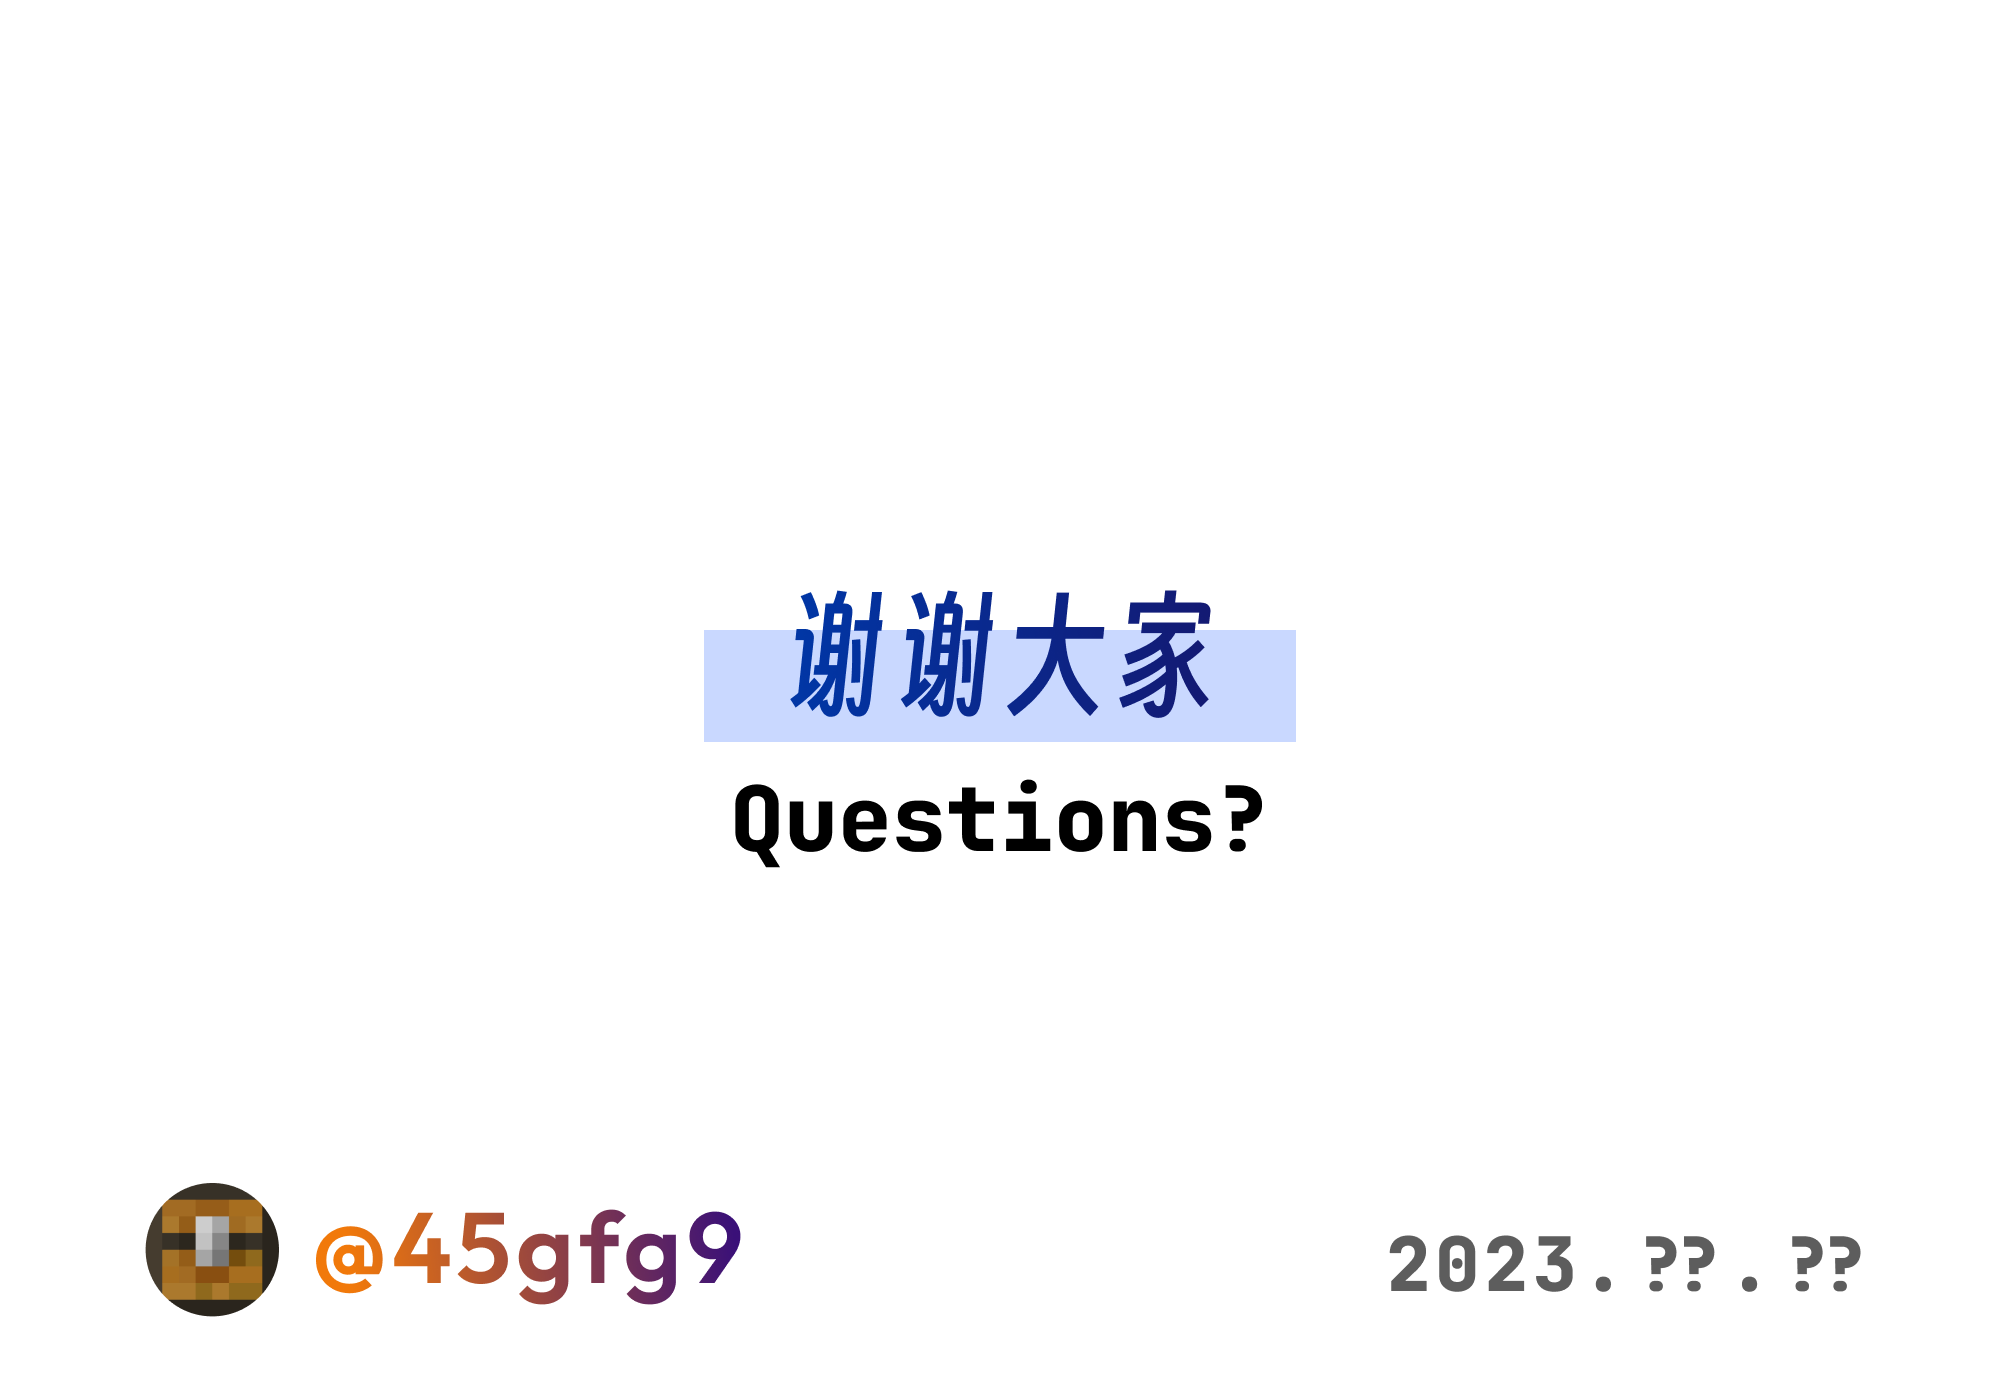
\includepdf{ending.png}

\end{document}
